%! app: Regular Languages, Context-free Languages
%! outcome: Formal definition of automata, Informal definition of automata, Nondeterminism, Classify language

Regular sets are not the end of the story
\begin{itemize}
    \item Many nice / simple / important sets are not regular
    \item Limitation of the finite-state automaton model: Can't ``count", Can only remember finitely far into the past,
    Can't backtrack, Must make decisions in ``real-time"
    \item We know actual computers are more powerful than this model...
\end{itemize}

The {\bf next} model of computation. Idea: allow some memory of unbounded size. How? 
\begin{itemize}
    \item To generalize regular expressions: {\bf context-free grammars}\\
    \item To generalize NFA: {\bf Pushdown automata}, which is like an NFA with access to a stack: 
    Number of states is fixed, number of entries in stack is unbounded. At each step
    (1) Transition to new state based on current state, letter read, and top letter of stack, then
    (2) (Possibly) push or pop a letter to (or from) top of stack. Accept a string iff
    there is some sequence of states and some sequence of stack contents 
    which helps the PDA processes the entire input string and ends in an accepting state.
\end{itemize}

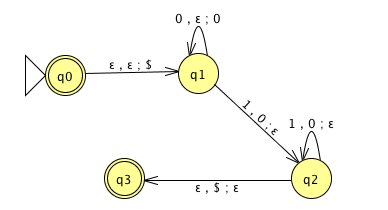
\includegraphics[width=4in]{../../resources/machines/Lect9PDA.png}
    
Trace the computation of this PDA on the input string $01$.

\vfill
    
Trace the computation of this PDA on the input string $011$.

\vfill
\newpage
{\bf Definition} A {\bf pushdown automaton} (PDA) is  specified by a  $6$-tuple $(Q, \Sigma, \Gamma, \delta, q_0, F)$
where $Q$ is the finite set of states, $\Sigma$ is the input alphabet,  $\Gamma$ is the stack alphabet,
\[
    \delta: Q \times \Sigma_\varepsilon  \times  \Gamma_\varepsilon \to \mathcal{P}( Q \times \Gamma_\varepsilon)
\]
is the transition function,  $q_0 \in Q$ is the start state, $F \subseteq  Q$ is the set of accept states.
    
\begin{multicols}{2}
    {\it Formal definition}
    
    \vspace{90pt}
    Draw the state diagram of a PDA with $\Sigma = \Gamma$.
    
    \columnbreak 
    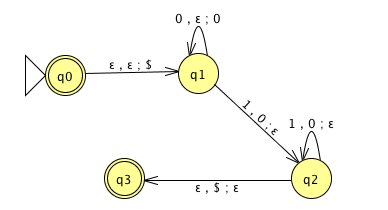
\includegraphics[height=100pt]{../../resources/machines/Lect9PDA.png}
    
    
    Draw the state diagram of a PDA with $\Sigma \cap \Gamma = \emptyset$.
    
\end{multicols}
    
\vspace{60pt}
